\documentclass[10pt]{article}

% ─── Packages ─────────────────────────────────────────────────────────────────
\usepackage[margin=1in]{geometry}
\usepackage{amsmath}
\usepackage{amssymb}
\usepackage{graphicx}
\usepackage{booktabs}
\usepackage{multirow}
\usepackage{array}
\usepackage{xcolor}
\usepackage{hyperref}
\usepackage{pgfplots}
\usepackage{pgfplotstable}
\usepackage{tikz}
\usetikzlibrary{positioning}
\usepackage{caption}
\usepackage{subcaption}
\usepackage{float}
\usepackage{enumitem}
\usepackage{microtype}
\usepackage{siunitx}
\usepackage{url}
\usepackage{cite}

\pgfplotsset{compat=1.18}

% ─── Hyperlink Styling ────────────────────────────────────────────────────────
\hypersetup{
    colorlinks=true,
    linkcolor=blue!60!black,
    citecolor=green!40!black,
    urlcolor=blue!60!black,
}

% ─── Custom colours ───────────────────────────────────────────────────────────
\definecolor{btreeblue}{RGB}{41, 98, 175}
\definecolor{lsmgreen}{RGB}{27, 140, 60}
\definecolor{cliffgray}{RGB}{120, 120, 120}
\definecolor{stressred}{RGB}{192, 40, 40}
\definecolor{recoveryamber}{RGB}{200, 130, 0}

% ─── Title ────────────────────────────────────────────────────────────────────
\title{\textbf{Workload Shifter: Evaluating Temporal Response to Database Workload Transitions}\\[4pt]
       \large \textit{A Five-Configuration Pilot Study}}

\author{
  \textit{Research manuscript draft}\\[2pt]
  \small \texttt{[author list pending]}
}

\date{October 2026}

% ─── Document ─────────────────────────────────────────────────────────────────
\begin{document}
\maketitle
\begin{abstract}
Database benchmarks commonly summarize performance under fixed workloads, whereas deployed workloads change over time. We present Workload Shifter, a three-phase protocol that measures performance before, during, and after a controlled change in operation mix and key popularity. Its paired return-to-baseline measure complements whole-run throughput and tail latency without conflating recovery-phase performance with time-to-recovery. We apply the protocol to three archived runs of five database configurations. The pilot shows that recorded call-rate rankings and return-to-baseline ratios can diverge: RocksDB has the highest mean whole-run call rate, yet a variable return-phase deficit, while MySQL and PostgreSQL call rates return near their initial levels. These are exploratory call-level observations. The archived harness did not record operation success, and PostgreSQL's near-zero update counters and large rollback counts leave its write-heavy phase unverified. The study therefore demonstrates the protocol and identifies the measurements required for a definitive cross-system comparison; it does not establish a storage-architecture ranking.
\end{abstract}
\noindent\textbf{Keywords:} Workload Shifter; dynamic benchmarks; temporal resilience; storage engines; recovery; run-level analysis.

\section{Introduction}
B$^+$-trees and log-structured merge trees make different choices about buffering, updates, and background maintenance \cite{oneil1996,graefe2010}. Benchmarks such as YCSB permit controlled comparisons under fixed workload profiles \cite{cooper2010}. A transition poses a further question: how does a system respond when operation mix and key popularity change, and what level of performance does the original workload attain when it returns? A single average over the complete run cannot answer that question.

Workload Shifter makes the transition an explicit experimental unit. It specifies a baseline, a perturbation, and a return phase within one run; retains the phase trajectory; and pairs each run's return-phase rate with its own baseline. This design exposes the distinction among absolute rate, stability under perturbation, and short-horizon return performance. We report a pilot application to five end-to-end database configurations, with uncertainty computed across runs rather than across second-level samples. The RUM conjecture motivates attention to read, update, and space costs \cite{athanassoulis2016}, although the present data do not measure their amplification factors comparably.

Time-varying workloads are established prior art: Dyn-YCSB varies YCSB parameters over time to evaluate adaptive frameworks \cite{sidhanta2019}. Workload Shifter's contribution is narrower and operationally specific: an explicit return-to-baseline phase, paired within-run comparison, and run-level presentation of the resulting trajectory across configurations. Its pilot is intended to demonstrate what that comparison reveals and where the current measurement harness falls short. Because the perturbation changes both operation mix and key popularity, the observed response is to their combined change.

\section{Background and Related Work}
\label{sec:background}
\subsection{Page-oriented and log-structured write paths}
A B$^+$-tree organizes records in sorted pages so a point lookup descends from a root through internal pages to a leaf. When a leaf is in memory, a lookup may need few device accesses; when it is absent, the engine must fetch the relevant page. An update also interacts with logging, page modification, and eventual page flushing. Concurrency control and recovery rules are part of the implementation, so the cost of a write cannot be inferred from the tree shape alone \cite{graefe2010,innodb}. MySQL/InnoDB and PostgreSQL both use B-tree indexes, but their heap organization, logging, and transaction machinery differ. They must therefore be treated as separate systems in the measurements.

An LSM design first places writes in memory and later persists sorted runs. Background merging reorganizes those runs and can move write cost out of the foreground operation. The resulting cost depends on level sizes, compaction policy, cache allocation, filters, and write rate \cite{oneil1996,luo2020}. RocksDB and LevelDB are embedded key-value libraries with different options and implementations. Cassandra uses LSM-derived storage inside a distributed database system. Its single-node client/server path includes work outside the storage engine, making an architectural class average across all three inappropriate.

These pathways suggest plausible responses to a write-heavy hot-key phase. Repeated updates to the same B-tree leaves may contend on shared pages or locks. LSM systems may absorb foreground writes temporarily and pay later at flush or compaction boundaries. Conversely, a return to uniform reads may encounter evicted blocks or still-running background work in either family. These are mechanisms to test, not diagnoses of the observed traces: the current JSON records contain no phase-aligned latch waits, cache evictions, or compaction durations.

\begin{figure}[htbp]
\centering
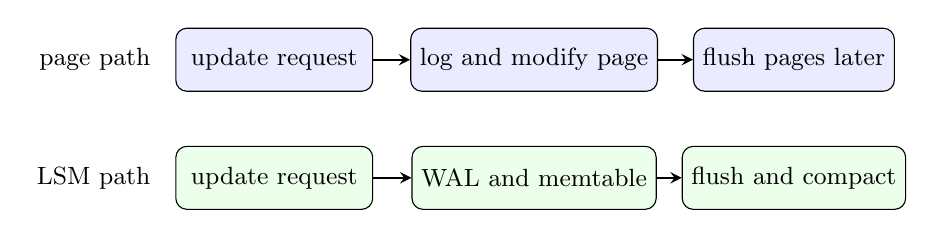
\begin{tikzpicture}[>=stealth, every node/.style={font=\small}]
\node[draw, rounded corners, fill=blue!8, minimum width=2.5cm, minimum height=.8cm] (bw) at (0,0) {update request};
\node[draw, rounded corners, fill=blue!8, minimum width=2.5cm, minimum height=.8cm] (blog) at (3.3,0) {log and modify page};
\node[draw, rounded corners, fill=blue!8, minimum width=2.5cm, minimum height=.8cm] (bdisk) at (6.6,0) {flush pages later};
\draw[->,thick] (bw)--(blog); \draw[->,thick] (blog)--(bdisk);
\node[draw, rounded corners, fill=green!8, minimum width=2.5cm, minimum height=.8cm] (lw) at (0,-1.5) {update request};
\node[draw, rounded corners, fill=green!8, minimum width=2.5cm, minimum height=.8cm] (lmem) at (3.3,-1.5) {WAL and memtable};
\node[draw, rounded corners, fill=green!8, minimum width=2.5cm, minimum height=.8cm] (lsst) at (6.6,-1.5) {flush and compact};
\draw[->,thick] (lw)--(lmem); \draw[->,thick] (lmem)--(lsst);
\node[anchor=east] at (-1.45,0) {page path};
\node[anchor=east] at (-1.45,-1.5) {LSM path};
\end{tikzpicture}
\caption{Conceptual write paths. Actual logging, durability, concurrency, and cache behavior depend on each engine's configuration. The diagram motivates measurements rather than assigning a cause to the current results.}
\label{fig:paths}
\end{figure}

\subsection{Amplification and changing workloads}
The RUM perspective describes a tension among read, update, and memory or space costs \cite{athanassoulis2016}. A design can reduce foreground write cost by retaining more in memory or performing later compaction, while a different design may pay more at update time and retain a simpler read path. Amplification is especially relevant during a workload shift because background work initiated by one phase may continue into the next. A brief benchmark can therefore mistake deferred work for an intrinsic saving unless it includes a drain or quiescence period.

YCSB made cross-system workload definitions central to cloud-serving benchmarks \cite{cooper2010}. Dyn-YCSB subsequently introduced time-varying workload parameters to evaluate adaptive systems \cite{sidhanta2019}. Research on filters and merge policies explains why LSM designs may behave differently as conditions change \cite{dayan2017,dayan2018}. Here the variable of interest is the transition's observed effect on each system and the extent to which the original workload's throughput returns. The two changing workload attributes remain coupled in this experiment, and our results do not isolate their separate effects.

\subsection{Scope of the comparison}
The five systems serve different use cases. MySQL and PostgreSQL are relational servers, Cassandra is a distributed database accessed through a driver, and RocksDB and LevelDB are embedded libraries. Comparing their end-to-end operation rates can inform deployment choices under the exact benchmark contract. It does not compare storage engines under identical call overhead, transaction semantics, or durability rules. Both perspectives are valuable, but each needs its own experimental setup and label. The current results belong to the end-to-end comparison.

\section{Study Design}
\label{sec:design}
The study compares whole-run throughput and P99 latency across five systems and asks whether throughput in the return-to-baseline phase matches the initial phase within each run. These are distinct outcomes: a system with high average throughput may still have a persistent post-shift deficit. Architectural explanations are evaluated as plausible mechanisms in the discussion, subject to the available cache, I/O, and contention evidence.

\begin{figure}[htbp]
\centering
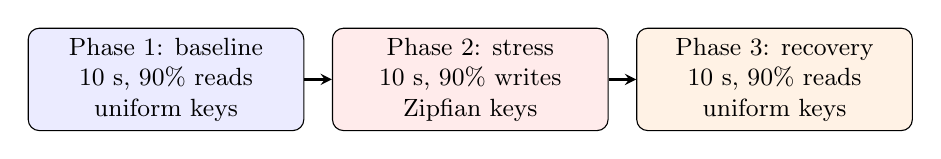
\begin{tikzpicture}[>=stealth, node distance=0.35cm, every node/.style={font=\small}]
\node[draw, rounded corners, fill=blue!8, minimum width=3.5cm, minimum height=1.3cm, align=center] (base) {Phase 1: baseline\\10 s, 90\% reads\\uniform keys};
\node[draw, rounded corners, fill=red!8, minimum width=3.5cm, minimum height=1.3cm, align=center, right=of base] (stress) {Phase 2: stress\\10 s, 90\% writes\\Zipfian keys};
\node[draw, rounded corners, fill=orange!10, minimum width=3.5cm, minimum height=1.3cm, align=center, right=of stress] (recover) {Phase 3: recovery\\10 s, 90\% reads\\uniform keys};
\draw[->, thick] (base) -- (stress);
\draw[->, thick] (stress) -- (recover);
\end{tikzpicture}
\caption{The Workload Shifter transition implemented by the benchmark harness. One-second call-rate and latency summaries are recorded throughout the run.}
\label{fig:design}
\end{figure}

\subsection{Experimental configuration}
According to the study's hardware record, the runs used an AWS EC2 \texttt{r6idn.2xlarge}. AWS lists this type with 8 vCPUs, 64~GiB of RAM, and one 474-GB local NVMe SSD \cite{awsr6idn}.

The repository's EC2 provisioning script attempts to mount local NVMe storage and installs MySQL, PostgreSQL, Cassandra, RocksDB, and LevelDB from system packages. The results do not contain an instance identifier, mount manifest, operating-system release, package-version list, or effective database settings. Thus the provisioning script documents intended setup, while actual file placement and software versions remain unverified from the archived runs.

\begin{table}[htbp]
\centering\small
\caption{Configuration facts and provenance for the pilot. ``Unrecorded'' means the effective setting cannot be reconstructed from the archived run files.}
\label{tab:configuration}
\begin{tabular}{@{}p{.27\linewidth}p{.62\linewidth}@{}}\toprule
Item & Supported description \\ \midrule
Host hardware & Author-reported \texttt{r6idn.2xlarge}; AWS lists 8 vCPUs, 64~GiB RAM, and one 474-GB NVMe SSD. \\
Operating system & EC2 setup script uses \texttt{apt}; exact distribution and release unrecorded. \\
Database versions & Exact installed MySQL, PostgreSQL, Cassandra, RocksDB, LevelDB, and driver versions unrecorded. \\
Worker and workload & Per-engine scripts invoke \texttt{--chaos}; harness defaults to one worker and a 1,024-byte repeated-character write value. Each nominal phase lasts 10~s. \\
Dataset and access & Scripts default to 10 million keys; actual command-line invocation and dataset checksum unrecorded. Baseline and return are 90\% reads with uniform keys; stress is 90\% writes with Zipfian $\theta=0.99$. \\
Managed caches and memory & Effective EC2 buffer-pool, shared-buffer, block-cache, and total-process limits unrecorded. The host has 64~GiB RAM; no 64-MB total-memory limit is established. \\
Durability and placement & Effective server durability settings and placement of embedded database files unrecorded. The EC2 setup script attempts NVMe mounts; completion is not logged in the result files. \\
\bottomrule\end{tabular}
\end{table}

The repository also contains a Docker Compose development setup with a 64-MB InnoDB buffer pool and 64-MB PostgreSQL shared-buffer setting. Those are database-managed allocations in a separate environment, not measurements of EC2 process memory. Memtables, block caches, server heaps, and the operating-system page cache can consume additional RAM. The Docker image tags and durability options must not be substituted for the unrecorded settings of the EC2 run.

The pilot comprises three consecutive runs per configuration. The run scripts specify a fixed configuration order, with MySQL and PostgreSQL service restarts before their respective three-run series. The study treats the complete adapter and database path as the tested configuration, including client/server communication where present.



The sampler emits 30 approximately one-second points per run. For descriptive phase analysis, we take points 1--10, 11--20, and 21--30 as the three nominal phases. A sampling interval may straddle a transition, and elapsed timestamps drift slightly beyond 30 seconds. Exact phase-aligned estimates require explicit boundary timestamps and operation counts. The whole-run P99 comes from the run-level latency summary; a mean of one-second P99 values would not equal that quantile.

\section{Experimental Implementation}
\label{sec:implementation}
\subsection{Harness and operation generation}
The C++ harness exposes one adapter interface for reads, writes, scans, and metric collection. In the archived \texttt{--chaos} mode it runs the three phases in Figure~\ref{fig:design} sequentially. Every worker repeatedly chooses a read or write according to the current phase percentage, chooses a key from the current distribution, calls the adapter, and records the elapsed operation time. A uniform draw spans the configured key range. The Zipfian generator uses an exponent of $\theta=0.99$ by default. The code seeds its random number generators from \texttt{std::random\_device}; seeds are not saved in the result JSON, so replaying the exact key stream is not possible from the archive alone.

The default payload is a 1,024-byte string of the same character, not a random byte sequence. It is passed to write operations. This matters for compression and physical-space comparisons: highly compressible data may yield different device bytes from realistic application values. The code times a call around each operation using a monotonic clock and stores integer microseconds. The configuration used to obtain each archived JSON file is inferred from the run scripts and defaults, since the JSON format does not store the command line or effective engine settings.

Each worker accumulates latency samples locally and flushes them to shared statistics after 1,000 operations or at the end of its phase. A monitor thread wakes at roughly one-second intervals and records interval throughput and latency summaries. The asynchronous flush and sampler clocks are not synchronized to phase boundaries. A sample near 10 or 20 seconds may mix work from adjacent phases, and a short-lived interval can contain incomplete worker buffers. These implementation details motivate the boundary sensitivity check in Section~\ref{sec:results}.

\subsection{Database state and execution order}
The scripts run RocksDB, LevelDB, MySQL, PostgreSQL, and Cassandra in that order, with three sequential runs for each system. The MySQL and PostgreSQL scripts restart their services before the respective series. Their adapters check whether a table already contains enough rows before seeding. The RocksDB and LevelDB adapters check for an existing key before seeding. Thus later runs can inherit populated data and potentially altered cache or compaction state; a service restart does not by itself establish a cold disk cache. The current archive lacks a per-run state manifest. This is a direct reason to interpret the three runs as a small, possibly dependent sequence rather than fully randomized replicates.

Embedded engines share a database handle among workers, whereas networked engines create separate client connections. The comparison consequently includes client, protocol, and server costs for some systems but library-call costs for others. A future engine-focused experiment could put each system behind a comparable client/server wrapper, while retaining a separate deployment-focused comparison that measures the systems as operators actually use them.

\subsection{System and engine telemetry}
The run scripts launch \texttt{dstat} alongside each workload and store a CSV file for each engine and run. Those CSVs provide coarse CPU, memory, disk, and network context. Their clocks are separate from the JSON sampler, and no synchronized event markers identify phase boundaries within the CSVs. The present analysis therefore does not correlate individual throughput dips with a specific disk or CPU event. Such attribution would require clock alignment, baseline load measurement, and repeated coincidence across independent runs.

The adapters also collect engine-specific counters after a run. MySQL queries global status and table-size metadata; PostgreSQL queries its statistics and relation sizes; RocksDB and LevelDB expose selected properties; Cassandra exposes its own metrics. Some counters are cumulative since server start or include work unrelated to the measured interval. A valid cross-system rate requires a before/after counter difference over a common window, not a single final snapshot. In particular, the zero-filled amplification fields in the JSON files cannot be interpreted as measured zero cost.

\section{Metrics and Measurement Semantics}
\label{sec:metrics}
\subsection{Throughput and tail latency}
The recorded call rate divides returned adapter calls by elapsed wall time:
\begin{equation}
T_{\mathrm{call}}=\frac{N_{\mathrm{returned\ calls}}}{t_{\mathrm{end}}-t_{\mathrm{start}}}\quad\mathrm{calls/s}.
\end{equation}
The archived JSON stores this rate directly. The harness increments its count when an adapter call returns; it does not record whether the database operation succeeded. We therefore refer to \emph{recorded call rate}, not successful-operation throughput. The harness computes latency summaries from the recorded call times. Its percentile procedure sorts the run's samples and chooses the element at the integer index corresponding to the requested percentage. P99 describes the 99th percentile of recorded call durations under that implementation and includes only work inside the timed adapter call.

A one-second P99 summarizes calls returned in that interval. Averaging 30 such values would give equal weight to busy and quiet seconds and would not reproduce the quantile of all calls in a run. We use the run-level P99 for Table~\ref{tab:observed}. Interval P99 traces remain useful for locating transient spikes, subject to the number of calls observed in each interval.

\subsection{Recovery}
The paired call-rate ratio $R_{er}$ in Section~\ref{sec:statistics} describes how the post-stress phase compares with its own initial baseline. The paired difference $D_{er}$ retains calls/s units and helps interpret a ratio with an unusually low denominator. Neither quantity measures the time required to recover: that outcome would require a prespecified threshold and a longer observation period. The ten-second return phase supports only a short-horizon comparison.

\section{Estimands and Statistical Analysis}
\label{sec:statistics}
For configuration $e$ and run $r$, let $T_{er}$ be the recorded whole-run call rate, $Q_{er}$ its whole-run P99 call latency, and $\bar T_{erp}$ the arithmetic mean of ten sampled call rates in phase $p$. Our paired short-horizon return measure is
\begin{equation}
R_{er}=\frac{\bar T_{er3}}{\bar T_{er1}},\qquad
D_{er}=\bar T_{er3}-\bar T_{er1}.
\end{equation}
$R=1$ denotes return to the initial call rate; it does not measure time-to-recovery. A ratio above one can reflect warmup, drift, or a faster return phase. We report the arithmetic mean of the three run-level ratios, never the ratio of pooled phase means.

For each scalar metric $x_r$ we show $\bar x\pm t_{0.975,2}s_x/\sqrt{3}$, where $s_x$ is the sample standard deviation and $t_{0.975,2}=4.303$. These intervals describe between-run dispersion under an approximate independent-run model. We do not treat the 30 time points within each run as independent replicates, perform ranking significance tests, or infer equivalence from overlapping intervals. The limitations of three consecutive runs are discussed in Section~\ref{sec:threats}.

\section{Results}
\label{sec:results}
\newcommand{\MySQLRecoveryPlot}{\addplot[only marks,mark=square*,color=btreeblue,mark size=2.4pt] coordinates {(1.9,1.006) (2.0,1.002) (2.1,0.971)};}
\newcommand{\PostgreSQLRecoveryPlot}{\addplot[only marks,mark=triangle*,color=cliffgray,mark size=2.4pt] coordinates {(2.9,1.007) (3.0,1.006) (3.1,1.019)};}
\newcommand{\RocksDBRecoveryPlot}{\addplot[only marks,mark=*,color=lsmgreen,mark size=2.4pt] coordinates {(0.9,0.474) (1.0,0.717) (1.1,1.004)};}
\newcommand{\LevelDBRecoveryPlot}{\addplot[only marks,mark=diamond*,color=green!45!black,mark size=2.4pt] coordinates {(3.9,3.066) (4.0,1.010) (4.1,1.004)};}
\newcommand{\CassandraRecoveryPlot}{\addplot[only marks,mark=pentagon*,color=orange!75!black,mark size=2.4pt] coordinates {(4.9,1.343) (5.0,1.025) (5.1,1.007)};}
\newcommand{\MySQLInteriorRecovery}{0.99}
\newcommand{\PostgreSQLInteriorRecovery}{1.01}
\newcommand{\RocksDBInteriorRecovery}{0.77}
\newcommand{\LevelDBInteriorRecovery}{2.26}
\newcommand{\CassandraInteriorRecovery}{1.13}
% Generated by python3 scripts/paper_analysis.py; do not edit by hand.
\begin{table}[htbp]
\centering\small
\caption{Thirty-second Workload Shifter pilot runs (three runs per configuration). Values are recorded completed adapter-call rates and call latencies; operation success was not recorded. Means and descriptive two-sided 95\% Student-$t$ intervals use runs as the unit. Recovery is the within-run Phase 3/Phase 1 call-rate ratio. P99 is the whole-run value.}
\label{tab:observed}
\begin{tabular}{@{}lrrr@{}}\toprule
Configuration & Call rate (calls/s) & Whole-run P99 ($\mu$s) & Return/baseline \\ \midrule
MySQL & $12,013\pm187$ & $108.7\pm5.2$ & $0.99\pm0.05$ \\
PostgreSQL & $18,120\pm297$ & $70.7\pm3.8$ & $1.01\pm0.02$ \\
RocksDB & $86,648\pm22,772$ & $29.3\pm1.4$ & $0.73\pm0.66$ \\
LevelDB & $58,013\pm41,060$ & $371.3\pm1488.0$ & $1.69\pm2.95$ \\
Cassandra & $3,410\pm684$ & $545.7\pm277.6$ & $1.12\pm0.47$ \\
\bottomrule\end{tabular}
\end{table}
\begin{table}[htbp]
\centering\small
\caption{Mean recorded adapter-call rate in each nominal phase, averaged within runs and then across three runs (mean $\pm$ between-run standard deviation, calls/s). Time points within a run are not independent replicates.}
\label{tab:phases}
\begin{tabular}{@{}lrrr@{}}\toprule
Configuration & Baseline & Stress & Return \\ \midrule
MySQL & $11,135\pm50$ & $13,846\pm51$ & $11,058\pm192$ \\
PostgreSQL & $17,954\pm187$ & $18,265\pm125$ & $18,145\pm122$ \\
RocksDB & $85,749\pm29,304$ & $115,747\pm1,072$ & $57,832\pm3,839$ \\
LevelDB & $63,277\pm33,210$ & $29,504\pm12,778$ & $80,888\pm4,047$ \\
Cassandra & $3,249\pm563$ & $3,398\pm181$ & $3,584\pm95$ \\
\bottomrule\end{tabular}
\end{table}


\begin{figure}[htbp]
\centering
\begin{tikzpicture}
\begin{axis}[width=.9\linewidth,height=6.2cm,xmin=1,xmax=30,ymin=0,ymax=2.2,
 xlabel={Nominal one-second interval},ylabel={Call rate / paired baseline mean},
 grid=major,grid style={dotted,gray!40},legend style={font=\scriptsize,at={(0.5,-0.22)},anchor=north,legend columns=5},
 tick label style={font=\footnotesize},label style={font=\footnotesize}]
\addplot[btreeblue,thick] table[x=second,y=mysql,col sep=space] {paper_timeseries.dat};
\addlegendentry{MySQL}
\addplot[cliffgray,thick,dashed] table[x=second,y=postgresql,col sep=space] {paper_timeseries.dat};
\addlegendentry{PostgreSQL}
\addplot[lsmgreen,thick] table[x=second,y=rocksdb,col sep=space] {paper_timeseries.dat};
\addlegendentry{RocksDB}
\addplot[green!45!black,thick,dotted] table[x=second,y=leveldb,col sep=space] {paper_timeseries.dat};
\addlegendentry{LevelDB}
\addplot[orange!75!black,thick,dashdotted] table[x=second,y=cassandra,col sep=space] {paper_timeseries.dat};
\addlegendentry{Cassandra}
\addplot[black!60,densely dashed] coordinates {(10.5,0)(10.5,2.2)};
\addplot[black!60,densely dashed] coordinates {(20.5,0)(20.5,2.2)};
\end{axis}
\end{tikzpicture}
\caption{One-second recorded call rate normalized to each run's mean baseline rate, then averaged across three runs. Dashed vertical lines denote nominal phase changes. Table~\ref{tab:phases} reports between-run variability.}
\label{fig:temporal}
\end{figure}

RocksDB records the highest mean whole-run call rate, 86,648 calls/s; its three values range from 79,778 to 97,057. LevelDB's values range from 38,980 to 68,762 calls/s, with a conspicuous latency outlier: its whole-run P99 is 1,063~$\mu$s in the first run and 26 and 25~$\mu$s in the next two. Table~\ref{tab:observed} reports these quantities as pilot observations of the instrumented call paths. It does not rank successful database operations.

\begin{figure}[htbp]
\centering
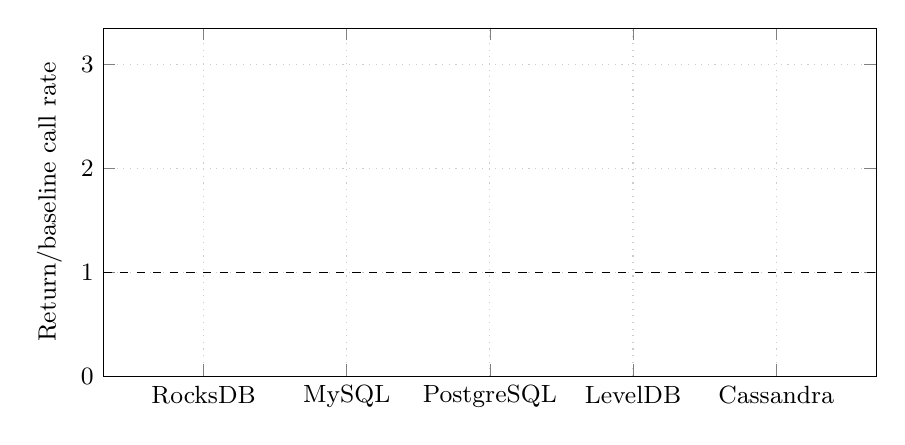
\begin{tikzpicture}
\begin{axis}[width=.94\linewidth,height=6cm,xmin=.3,xmax=5.7,ymin=0,ymax=3.35,
  xtick={1,2,3,4,5},xticklabels={RocksDB,MySQL,PostgreSQL,LevelDB,Cassandra},ylabel={Return/baseline call rate},
  grid=major,grid style={dotted,gray!40},tick label style={font=\small},label style={font=\small}]
\addplot[black,dashed,domain=.3:5.7] {1};
\RocksDBRecoveryPlot
\MySQLRecoveryPlot
\PostgreSQLRecoveryPlot
\LevelDBRecoveryPlot
\CassandraRecoveryPlot
\end{axis}
\end{tikzpicture}
\caption{Run-level return-to-baseline call-rate ratios for all five configurations. Horizontal offsets separate the three runs; the dashed line denotes equal call rates in the two read-heavy phases. Ratios are computed from the JSON one-second samples.}
\label{fig:recovery}
\end{figure}

The ratio estimates give a different picture from whole-run call rate. RocksDB's mean return-to-baseline ratio is 0.73 and varies across runs. MySQL and PostgreSQL call rates are near their initial levels, whereas LevelDB's ratio is driven upward by a slow first baseline run. Figure~\ref{fig:recovery} shows all three ratios for each configuration rather than hiding this variation in a single summary.

\section{Discussion}
\label{sec:discussion}
\subsection{Absolute rate, perturbation response, and return performance}
Workload Shifter makes three different aspects of temporal behavior visible. Whole-run call rate describes aggregate completed work; the stress-phase rate describes behavior under a different mix and key distribution; and the paired return ratio describes how the original read-heavy workload performs after that change. These quantities need not move together. The rate in the stress phase should not be called ``retention'' of baseline performance because the operations being executed have changed. Likewise, a return ratio close to one says that the two ten-second read-heavy phases have similar average call rates; it says nothing about the elapsed time needed to cross a recovery threshold.

Table~\ref{tab:phases} and Figure~\ref{fig:temporal} show the divergence in the pilot. RocksDB's mean recorded call rate rises from about 85,749 calls/s in the baseline to 115,747 in the skewed write-heavy phase, then falls to 57,832 in the return phase. The high aggregate rate in Table~\ref{tab:observed} therefore coexists with a lower immediate return-phase rate. Figure~\ref{fig:recovery} shows that its three paired return ratios range from 0.47 to 1.00. The ratio's variation matters as much as its mean: a lower initial phase can raise a ratio even when the return-phase rate does not improve.

MySQL's phase means are approximately 11,135, 13,846, and 11,058 calls/s; PostgreSQL's are 17,954, 18,265, and 18,145. Their call-rate ratios cluster near one. These traces do not establish equivalent successful read or write performance: the interfaces and operation semantics differ, and the PostgreSQL write path is invalid for the configured payload. The contrast is nevertheless useful methodologically. A study that reported only whole-run rates would miss the difference between a high aggregate rate and a short-horizon return deficit.

LevelDB's first run has a much slower baseline than its other two runs and a much larger return ratio. It also has a whole-run P99 of 1,063~$\mu$s, versus 26 and 25~$\mu$s in runs two and three. This heterogeneity prevents a precise summary of its typical tail behavior from three runs. Cassandra's call-rate phase means increase modestly through the run, but its server and driver path is qualitatively different from the two embedded libraries. It is presented as a separate configuration rather than as an LSM-class observation.

Excluding the first and last one-second sample of each nominal phase gives mean return ratios of \MySQLInteriorRecovery{} for MySQL, \PostgreSQLInteriorRecovery{} for PostgreSQL, \RocksDBInteriorRecovery{} for RocksDB, \LevelDBInteriorRecovery{} for LevelDB, and \CassandraInteriorRecovery{} for Cassandra. The directional call-rate pattern remains, while LevelDB becomes more sensitive to its atypical first run. This sensitivity check addresses phase-boundary mixing, not carry-over or operation validity.

\subsection{Mechanisms and the RUM perspective}
The phase traces motivate several possible explanations for later measurement. Compaction or cache-state changes could overlap a return phase in an LSM implementation; skew might change locality in a B-tree implementation; and logging or checkpoint work might cross a phase boundary. The available end-of-run counters cannot identify the timing or size of any of these effects. We therefore do not attribute the RocksDB call-rate deficit to compaction, eviction, or a particular synchronization mechanism.

Read, update, and memory costs remain relevant to why a system responds to a transition \cite{athanassoulis2016}. The present results do not measure a comparable read, write, or space amplification factor across systems. RUM supplies a framework for asking which costs move when the workload changes, while the empirical contribution here is the phase-aware measurement protocol and its exploratory call-level application.

\section{Threats to Validity}
\label{sec:threats}
\subsection{Internal validity}
The three runs for each configuration were consecutive rather than randomized, and adapters can reuse populated state. Persistent page cache, compaction backlog, or background server activity may therefore change between runs. The interval sampler wakes independently of workload phase changes, so points near a boundary may mix operations from adjacent phases. The separate \texttt{dstat} CSVs lack synchronized phase markers; some contain many more records than a 30-second run. They cannot be used to assign a throughput change to a particular CPU or disk event in this study. Three potentially dependent runs also make the Student-$t$ intervals descriptive rather than strong coverage guarantees. Neither per-second samples nor interpolated values supply additional independent runs.

\subsection{Construct validity}
The benchmark measures returned adapter calls, not verified successful operations. Adapter methods generally discard database status results, and the JSON files contain no common attempted/successful-operation counters. PostgreSQL requires particular caution: the adapter creates a \texttt{VARCHAR(255)} value column if the table is absent, whereas the EC2 setup script creates a \texttt{TEXT} column beforehand. The harness sends 1,024-byte values, and the archive does not record which schema was present. The PostgreSQL snapshots report almost no updated tuples and large, increasing rollback counts, consistent with many failed writes but insufficient to identify their cause. Its write-heavy call rate cannot be interpreted as successful-update throughput or compared directly with other systems' write throughput.

The operation contracts also differ. MySQL uses \texttt{REPLACE INTO}, PostgreSQL uses \texttt{UPDATE}, and the embedded engines use \texttt{Put}; their write semantics and logging costs are not identical. RocksDB and LevelDB execute within the benchmark process, whereas MySQL, PostgreSQL, and Cassandra include client/server communication. Cassandra also includes distributed-database machinery on a single node. This is an end-to-end configuration study, not an isolated comparison of B-tree and LSM-tree algorithms. Durability settings, effective cache allocations, and several database versions were not archived. The Docker development settings do not establish the EC2 settings. Amplification fields that contain zero or use unmatched end-of-run counters do not measure zero amplification.

\subsection{External validity}
The pilot uses one author-reported host type, one nominal 10-million-key dataset, one worker, one payload, and ten-second phases. The repeated-character write value is highly compressible. Results may differ with realistic values, longer bursts, different concurrency, a working set that exceeds managed caches, or a different storage and network path. The ten-second return phase cannot establish time-to-recovery or long-term stability. The missing capacity, concurrency, payload, and amplification datasets are additional limits on the breadth of this manuscript's empirical claims.

\section{Future Work}
The present three-phase experiment changes write proportion and key skew together. A follow-up study should vary these factors separately, include a no-shift control, and extend the recovery window until background maintenance and throughput stabilize. Recording phase boundaries, operation outcomes, and read- and write-specific latency distributions would permit a time-to-recovery endpoint rather than only a phase-average ratio. Repeating the experiment in randomized fresh-state blocks on a documented machine would also separate workload response from execution-order and carry-over effects.

A broader architectural comparison requires the capacity, concurrency, and payload sweeps originally envisaged for this project. Each sweep should control effective memory use and durability semantics, pair engine counters with device-level measurements, and state whether the comparison targets a storage engine or the complete deployed system. Write and space amplification deserve a separate accounting study that includes deferred compaction or checkpoint activity. These additions would test proposed mechanisms without treating an end-of-run counter as a causal explanation.

\section{Conclusion}
Workload Shifter provides a repeatable baseline--perturbation--return protocol and a paired, run-level measure of short-horizon return performance. Its pilot illustrates why temporal response deserves a place beside whole-run rate: RocksDB records the highest aggregate call rate in these files but a variable return-phase deficit, while MySQL and PostgreSQL call rates return near baseline. The ten-second return phase does not measure time-to-recovery.

The archival harness did not verify operation success, and the PostgreSQL counters make its write-heavy result particularly uncertain. Consequently, the observed call-level contrast is a demonstration of the protocol rather than an architectural performance ranking. A definitive comparison requires validated operations, documented configurations, independent runs, and phase-aligned system measurements. The same framework can then accommodate the capacity, concurrency, payload, and amplification dimensions when their raw results are available and technically sound.

\noindent\textbf{Data and code availability.} The per-run JSON files are in \texttt{results/}. The script \path{scripts/paper_analysis.py} generates Tables~\ref{tab:observed} and~\ref{tab:phases}, Figure~\ref{fig:temporal}'s data, and the recovery plot coordinates.

\begin{thebibliography}{14}

\bibitem{awsr6idn}
Amazon Web Services, ``Amazon EC2 R6i and R6idn instances,'' \url{https://aws.amazon.com/ec2/instance-types/r6i/}, accessed October 2026.

\bibitem{oneil1996}
P.~O'Neil, E.~Cheng, D.~Gawlick, and E.~O'Neil, ``The Log-Structured Merge-Tree (LSM-Tree),'' \textit{Acta Informatica}, vol.~33, no.~4, pp.~351--385, 1996.

\bibitem{athanassoulis2016}
M.~Athanassoulis, M.~S.~Kester, L.~M.~Maas, R.~Stoica, S.~Idreos, A.~Ailamaki, and M.~Callaghan, ``Designing Access Methods: The RUM Conjecture,'' in \textit{Proc. EDBT}, pp.~461--466, 2016.

\bibitem{rocksdb}
Facebook Inc., ``RocksDB: A persistent key-value store for fast storage environments,'' \url{https://rocksdb.org}, 2013 (ongoing).

\bibitem{leveldb}
J.~Dean and S.~Ghemawat, ``LevelDB,'' \url{https://github.com/google/leveldb}, 2011 (ongoing).

\bibitem{innodb}
Oracle Corp., ``InnoDB Storage Engine,'' \textit{MySQL 8.0 Reference Manual}, 2024.

\bibitem{luo2020}
C.~Luo and M.~J.~Carey, ``LSM-based Storage Techniques: A Survey,'' \textit{VLDB Journal}, vol.~29, pp.~393--418, 2020.

\bibitem{dayan2017}
N.~Dayan, M.~Athanassoulis, and S.~Idreos, ``Monkey: Optimal Navigable Key-Value Store,'' in \textit{Proc. SIGMOD}, pp.~79--94, 2017.

\bibitem{dayan2018}
N.~Dayan and S.~Idreos, ``Dostoevsky: Better Space-Time Trade-Offs for LSM-Tree Based Key-Value Stores via Adaptive Removal of Superfluous Merging,'' in \textit{Proc. SIGMOD}, pp.~505--520, 2018.

\bibitem{cooper2010}
B.~F.~Cooper, A.~Silberstein, E.~Tam, R.~Ramakrishnan, and R.~S.~Sears, ``Benchmarking Cloud Serving Systems with YCSB,'' in \textit{Proc. SoCC}, pp.~143--154, 2010.

\bibitem{sidhanta2019}
S.~Sidhanta, S.~Mukhopadhyay, and W.~Golab, ``Dyn-YCSB: Benchmarking Adaptive Frameworks,'' in \textit{Proc. IEEE World Congress on Services}, pp.~392--393, 2019, doi:10.1109/SERVICES.2019.00119.

\bibitem{graefe2010}
G.~Graefe, ``A Survey of B-Tree Locking Techniques,'' \textit{ACM Transactions on Database Systems (TODS)}, vol.~35, no.~3, pp.~1--26, 2010.

\bibitem{idreos2019}
S.~Idreos, N.~Dayan, W.~Qin, M.~Akmanalp, S.~Hilgard, A.~Ross, J.~Lennon, V.~Jain, H.~Gupta, D.~Li, and Z.~Zhu, ``Design Continuums and the Path Toward Self-Designing Key-Value Stores that Know and Learn,'' in \textit{Proc. CIDR}, 2019.

\bibitem{postgres2024}
The PostgreSQL Global Development Group, ``PostgreSQL Documentation,'' Version 16, 2024.

\end{thebibliography}

\end{document}
